\documentclass[twoside]{book}

% Packages required by doxygen
\usepackage{fixltx2e}
\usepackage{calc}
\usepackage{doxygen}
\usepackage[export]{adjustbox} % also loads graphicx
\usepackage{graphicx}
\usepackage[utf8]{inputenc}
\usepackage{makeidx}
\usepackage{multicol}
\usepackage{multirow}
\PassOptionsToPackage{warn}{textcomp}
\usepackage{textcomp}
\usepackage[nointegrals]{wasysym}
\usepackage[table]{xcolor}

% Font selection
\usepackage[T1]{fontenc}
\usepackage[scaled=.90]{helvet}
\usepackage{courier}
\usepackage{amssymb}
\usepackage{sectsty}
\renewcommand{\familydefault}{\sfdefault}
\allsectionsfont{%
  \fontseries{bc}\selectfont%
  \color{darkgray}%
}
\renewcommand{\DoxyLabelFont}{%
  \fontseries{bc}\selectfont%
  \color{darkgray}%
}
\newcommand{\+}{\discretionary{\mbox{\scriptsize$\hookleftarrow$}}{}{}}

% Page & text layout
\usepackage{geometry}
\geometry{%
  a4paper,%
  top=2.5cm,%
  bottom=2.5cm,%
  left=2.5cm,%
  right=2.5cm%
}
\tolerance=750
\hfuzz=15pt
\hbadness=750
\setlength{\emergencystretch}{15pt}
\setlength{\parindent}{0cm}
\setlength{\parskip}{3ex plus 2ex minus 2ex}
\makeatletter
\renewcommand{\paragraph}{%
  \@startsection{paragraph}{4}{0ex}{-1.0ex}{1.0ex}{%
    \normalfont\normalsize\bfseries\SS@parafont%
  }%
}
\renewcommand{\subparagraph}{%
  \@startsection{subparagraph}{5}{0ex}{-1.0ex}{1.0ex}{%
    \normalfont\normalsize\bfseries\SS@subparafont%
  }%
}
\makeatother

% Headers & footers
\usepackage{fancyhdr}
\pagestyle{fancyplain}
\fancyhead[LE]{\fancyplain{}{\bfseries\thepage}}
\fancyhead[CE]{\fancyplain{}{}}
\fancyhead[RE]{\fancyplain{}{\bfseries\leftmark}}
\fancyhead[LO]{\fancyplain{}{\bfseries\rightmark}}
\fancyhead[CO]{\fancyplain{}{}}
\fancyhead[RO]{\fancyplain{}{\bfseries\thepage}}
\fancyfoot[LE]{\fancyplain{}{}}
\fancyfoot[CE]{\fancyplain{}{}}
\fancyfoot[RE]{\fancyplain{}{\bfseries\scriptsize Generated by Doxygen }}
\fancyfoot[LO]{\fancyplain{}{\bfseries\scriptsize Generated by Doxygen }}
\fancyfoot[CO]{\fancyplain{}{}}
\fancyfoot[RO]{\fancyplain{}{}}
\renewcommand{\footrulewidth}{0.4pt}
\renewcommand{\chaptermark}[1]{%
  \markboth{#1}{}%
}
\renewcommand{\sectionmark}[1]{%
  \markright{\thesection\ #1}%
}

% Indices & bibliography
\usepackage{natbib}
\usepackage[titles]{tocloft}
\setcounter{tocdepth}{3}
\setcounter{secnumdepth}{5}
\makeindex

% Custom commands
\newcommand{\clearemptydoublepage}{%
  \newpage{\pagestyle{empty}\cleardoublepage}%
}

\usepackage{caption}
\captionsetup{labelsep=space,justification=centering,font={bf},singlelinecheck=off,skip=4pt,position=top}

%===== C O N T E N T S =====

\begin{document}

% Titlepage & ToC
\pagenumbering{roman}
\begin{titlepage}
\vspace*{7cm}
\begin{center}%
{\Large Firmware\+Cliente-\/\+S\+O2\+T\+P1 \\[1ex]\large v1.\+0 }\\
\vspace*{1cm}
{\large Generated by Doxygen 1.8.11}\\
\end{center}
\end{titlepage}
\clearemptydoublepage
\tableofcontents
\clearemptydoublepage
\pagenumbering{arabic}

%--- Begin generated contents ---
\chapter{File Index}
\section{File List}
Here is a list of all files with brief descriptions\+:\begin{DoxyCompactList}
\item\contentsline{section}{{\bf main.\+c} }{\pageref{main_8c}}{}
\end{DoxyCompactList}

\chapter{File Documentation}
\section{main.\+c File Reference}
\label{main_8c}\index{main.\+c@{main.\+c}}
{\ttfamily \#include $<$stdio.\+h$>$}\\*
{\ttfamily \#include $<$string.\+h$>$}\\*
{\ttfamily \#include $<$sys/socket.\+h$>$}\\*
{\ttfamily \#include $<$netinet/in.\+h$>$}\\*
{\ttfamily \#include $<$arpa/inet.\+h$>$}\\*
{\ttfamily \#include $<$unistd.\+h$>$}\\*
{\ttfamily \#include $<$sys/sysinfo.\+h$>$}\\*
{\ttfamily \#include $<$stdbool.\+h$>$}\\*
{\ttfamily \#include $<$fcntl.\+h$>$}\\*
{\ttfamily \#include $<$stdlib.\+h$>$}\\*
{\ttfamily \#include $<$sys/stat.\+h$>$}\\*
Include dependency graph for main.\+c\+:\nopagebreak
\begin{figure}[H]
\begin{center}
\leavevmode
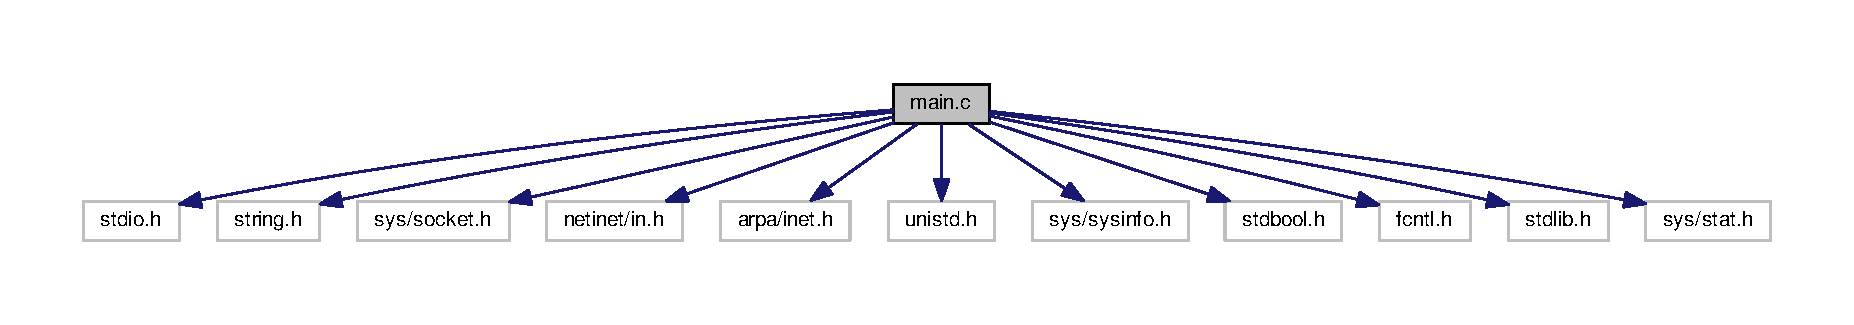
\includegraphics[width=350pt]{main_8c__incl}
\end{center}
\end{figure}
\subsection*{Macros}
\begin{DoxyCompactItemize}
\item 
\#define {\bf B\+U\+F\+F\+E\+R\+\_\+\+S\+I\+ZE}~1000
\item 
\#define {\bf P\+O\+R\+T\+U\+DP}~5521
\item 
\#define {\bf F\+I\+R\+M\+W\+A\+R\+E\+\_\+\+F\+I\+LE}~\char`\"{}./update\+\_\+file\char`\"{}
\item 
\#define {\bf F\+I\+L\+E\+\_\+\+B\+U\+F\+F\+E\+R\+\_\+\+S\+I\+ZE}~4000
\item 
\#define {\bf A\+R\+C\+H\+I\+V\+O\+\_\+\+I\+M\+A\+G\+EN}~\char`\"{}./archivo\+\_\+imagen\+\_\+cli.\+J\+PG\char`\"{}
\end{DoxyCompactItemize}
\subsection*{Functions}
\begin{DoxyCompactItemize}
\item 
long {\bf get\+\_\+uptime} ()
\begin{DoxyCompactList}\small\item\em Funcion que devuelve el uptime del sistema cuando es invacada. \end{DoxyCompactList}\item 
int {\bf update\+\_\+firmware} (int sockfd\+\_\+arg)
\begin{DoxyCompactList}\small\item\em Recibe mediante el socjet T\+CP de la comunicacion establecida un nuevo firmware. Luego de recibirlo satisfactoriamente se cierra el proceso actual y se ejecuta en nuevo firmaware perdiendo la conexion. \end{DoxyCompactList}\item 
int {\bf start\+\_\+scanning} (int sockfd\+\_\+arg2)
\begin{DoxyCompactList}\small\item\em Abre el archivo de imagen y lo envia al proceso servidor a traces del socket T\+CP abierto en la comunicacion establecida. \end{DoxyCompactList}\item 
int {\bf send\+\_\+telemetria} ()
\begin{DoxyCompactList}\small\item\em Abre un socket U\+DP con el numero de puerto especificado en la macro P\+O\+R\+T\+U\+DP. Obtiene la informacion de telemetria y la envia por el socket U\+DP recientemente abierto. \end{DoxyCompactList}\item 
int {\bf main} ()
\begin{DoxyCompactList}\small\item\em Programa cliente. Tiene como objetivo simular el firmaware del satelite que se conecta al programa servidor (Base Terrestre) y queda a la espera de ordenes del mismo. \end{DoxyCompactList}\end{DoxyCompactItemize}
\subsection*{Variables}
\begin{DoxyCompactItemize}
\item 
char {\bf firmware\+\_\+version} [20] = \char`\"{}1.\+0\char`\"{}
\item 
uint16\+\_\+t {\bf server\+\_\+port} = 5520
\item 
char {\bf ip\+\_\+server\+\_\+buff} [32] =\char`\"{}192.\+168.\+1.\+4\char`\"{}
\item 
char $\ast$ {\bf ip\+\_\+server} = N\+U\+LL
\item 
unsigned int {\bf retry\+\_\+time} =3
\end{DoxyCompactItemize}


\subsection{Macro Definition Documentation}
\index{main.\+c@{main.\+c}!A\+R\+C\+H\+I\+V\+O\+\_\+\+I\+M\+A\+G\+EN@{A\+R\+C\+H\+I\+V\+O\+\_\+\+I\+M\+A\+G\+EN}}
\index{A\+R\+C\+H\+I\+V\+O\+\_\+\+I\+M\+A\+G\+EN@{A\+R\+C\+H\+I\+V\+O\+\_\+\+I\+M\+A\+G\+EN}!main.\+c@{main.\+c}}
\subsubsection[{A\+R\+C\+H\+I\+V\+O\+\_\+\+I\+M\+A\+G\+EN}]{\setlength{\rightskip}{0pt plus 5cm}\#define A\+R\+C\+H\+I\+V\+O\+\_\+\+I\+M\+A\+G\+EN~\char`\"{}./archivo\+\_\+imagen\+\_\+cli.\+J\+PG\char`\"{}}\label{main_8c_ac9fcc8d0c149e86d5168674b6c519f63}
\index{main.\+c@{main.\+c}!B\+U\+F\+F\+E\+R\+\_\+\+S\+I\+ZE@{B\+U\+F\+F\+E\+R\+\_\+\+S\+I\+ZE}}
\index{B\+U\+F\+F\+E\+R\+\_\+\+S\+I\+ZE@{B\+U\+F\+F\+E\+R\+\_\+\+S\+I\+ZE}!main.\+c@{main.\+c}}
\subsubsection[{B\+U\+F\+F\+E\+R\+\_\+\+S\+I\+ZE}]{\setlength{\rightskip}{0pt plus 5cm}\#define B\+U\+F\+F\+E\+R\+\_\+\+S\+I\+ZE~1000}\label{main_8c_a6b20d41d6252e9871430c242cb1a56e7}
\index{main.\+c@{main.\+c}!F\+I\+L\+E\+\_\+\+B\+U\+F\+F\+E\+R\+\_\+\+S\+I\+ZE@{F\+I\+L\+E\+\_\+\+B\+U\+F\+F\+E\+R\+\_\+\+S\+I\+ZE}}
\index{F\+I\+L\+E\+\_\+\+B\+U\+F\+F\+E\+R\+\_\+\+S\+I\+ZE@{F\+I\+L\+E\+\_\+\+B\+U\+F\+F\+E\+R\+\_\+\+S\+I\+ZE}!main.\+c@{main.\+c}}
\subsubsection[{F\+I\+L\+E\+\_\+\+B\+U\+F\+F\+E\+R\+\_\+\+S\+I\+ZE}]{\setlength{\rightskip}{0pt plus 5cm}\#define F\+I\+L\+E\+\_\+\+B\+U\+F\+F\+E\+R\+\_\+\+S\+I\+ZE~4000}\label{main_8c_a09dbbd73a84cf772b421c6024b65b1fd}
\index{main.\+c@{main.\+c}!F\+I\+R\+M\+W\+A\+R\+E\+\_\+\+F\+I\+LE@{F\+I\+R\+M\+W\+A\+R\+E\+\_\+\+F\+I\+LE}}
\index{F\+I\+R\+M\+W\+A\+R\+E\+\_\+\+F\+I\+LE@{F\+I\+R\+M\+W\+A\+R\+E\+\_\+\+F\+I\+LE}!main.\+c@{main.\+c}}
\subsubsection[{F\+I\+R\+M\+W\+A\+R\+E\+\_\+\+F\+I\+LE}]{\setlength{\rightskip}{0pt plus 5cm}\#define F\+I\+R\+M\+W\+A\+R\+E\+\_\+\+F\+I\+LE~\char`\"{}./update\+\_\+file\char`\"{}}\label{main_8c_a6ef7baa1d4325116155fe508770ec911}
\index{main.\+c@{main.\+c}!P\+O\+R\+T\+U\+DP@{P\+O\+R\+T\+U\+DP}}
\index{P\+O\+R\+T\+U\+DP@{P\+O\+R\+T\+U\+DP}!main.\+c@{main.\+c}}
\subsubsection[{P\+O\+R\+T\+U\+DP}]{\setlength{\rightskip}{0pt plus 5cm}\#define P\+O\+R\+T\+U\+DP~5521}\label{main_8c_a1e95566bd8afa9c1606cbc245a42043a}


\subsection{Function Documentation}
\index{main.\+c@{main.\+c}!get\+\_\+uptime@{get\+\_\+uptime}}
\index{get\+\_\+uptime@{get\+\_\+uptime}!main.\+c@{main.\+c}}
\subsubsection[{get\+\_\+uptime()}]{\setlength{\rightskip}{0pt plus 5cm}long get\+\_\+uptime (
\begin{DoxyParamCaption}
{}
\end{DoxyParamCaption}
)}\label{main_8c_a02763bb54dc8e118437ec33a2889d1dd}


Funcion que devuelve el uptime del sistema cuando es invacada. 

\begin{DoxyReturn}{Returns}
Devuelve un long con el uptime 
\end{DoxyReturn}
\index{main.\+c@{main.\+c}!main@{main}}
\index{main@{main}!main.\+c@{main.\+c}}
\subsubsection[{main()}]{\setlength{\rightskip}{0pt plus 5cm}int main (
\begin{DoxyParamCaption}
{}
\end{DoxyParamCaption}
)}\label{main_8c_ae66f6b31b5ad750f1fe042a706a4e3d4}


Programa cliente. Tiene como objetivo simular el firmaware del satelite que se conecta al programa servidor (Base Terrestre) y queda a la espera de ordenes del mismo. 

\begin{DoxyReturn}{Returns}

\end{DoxyReturn}
\index{main.\+c@{main.\+c}!send\+\_\+telemetria@{send\+\_\+telemetria}}
\index{send\+\_\+telemetria@{send\+\_\+telemetria}!main.\+c@{main.\+c}}
\subsubsection[{send\+\_\+telemetria()}]{\setlength{\rightskip}{0pt plus 5cm}int send\+\_\+telemetria (
\begin{DoxyParamCaption}
{}
\end{DoxyParamCaption}
)}\label{main_8c_ae01dc0a40cb3aaf5c844abba47ffe1ec}


Abre un socket U\+DP con el numero de puerto especificado en la macro P\+O\+R\+T\+U\+DP. Obtiene la informacion de telemetria y la envia por el socket U\+DP recientemente abierto. 

\begin{DoxyReturn}{Returns}
Devuelve 0 si no se ha podido abrir el socket U\+DP. Devuelve 1 si la telemetria se ha enviado satisfactoriamente. No hay garantia de la integridad ni de la recepcion de los datos. 
\end{DoxyReturn}
\index{main.\+c@{main.\+c}!start\+\_\+scanning@{start\+\_\+scanning}}
\index{start\+\_\+scanning@{start\+\_\+scanning}!main.\+c@{main.\+c}}
\subsubsection[{start\+\_\+scanning(int sockfd\+\_\+arg2)}]{\setlength{\rightskip}{0pt plus 5cm}int start\+\_\+scanning (
\begin{DoxyParamCaption}
\item[{int}]{sockfd\+\_\+arg2}
\end{DoxyParamCaption}
)}\label{main_8c_a205c939d62529d045db32783efaf7a76}


Abre el archivo de imagen y lo envia al proceso servidor a traces del socket T\+CP abierto en la comunicacion establecida. 


\begin{DoxyParams}{Parameters}
{\em sockfd\+\_\+arg2} & Socketfd T\+CP abierto en la comunicacion cliente servidor \\
\hline
\end{DoxyParams}
\begin{DoxyReturn}{Returns}
Devuelve -\/1 cuando no se podido abrir el archivo de imagen a enviar para su lectura. Devuelve 1 al completar con exito el envio de la imagen. 
\end{DoxyReturn}
\index{main.\+c@{main.\+c}!update\+\_\+firmware@{update\+\_\+firmware}}
\index{update\+\_\+firmware@{update\+\_\+firmware}!main.\+c@{main.\+c}}
\subsubsection[{update\+\_\+firmware(int sockfd\+\_\+arg)}]{\setlength{\rightskip}{0pt plus 5cm}int update\+\_\+firmware (
\begin{DoxyParamCaption}
\item[{int}]{sockfd\+\_\+arg}
\end{DoxyParamCaption}
)}\label{main_8c_a57315c3f0ba1bb737f030bf10a4a655a}


Recibe mediante el socjet T\+CP de la comunicacion establecida un nuevo firmware. Luego de recibirlo satisfactoriamente se cierra el proceso actual y se ejecuta en nuevo firmaware perdiendo la conexion. 


\begin{DoxyParams}{Parameters}
{\em sockfd\+\_\+arg} & El socket de la comunicacion T\+CP establecida. \\
\hline
\end{DoxyParams}
\begin{DoxyReturn}{Returns}
Devuelve 0 si no se ha podido crear en el file system el archivo para la recepcion del firmware. Devuelve 1 en caso de que no se haya podido reiniciar el proceso cliente. 
\end{DoxyReturn}


\subsection{Variable Documentation}
\index{main.\+c@{main.\+c}!firmware\+\_\+version@{firmware\+\_\+version}}
\index{firmware\+\_\+version@{firmware\+\_\+version}!main.\+c@{main.\+c}}
\subsubsection[{firmware\+\_\+version}]{\setlength{\rightskip}{0pt plus 5cm}char firmware\+\_\+version[20] = \char`\"{}1.\+0\char`\"{}}\label{main_8c_acc4ef5efef44f2ed8aff7cf818e27f47}
\index{main.\+c@{main.\+c}!ip\+\_\+server@{ip\+\_\+server}}
\index{ip\+\_\+server@{ip\+\_\+server}!main.\+c@{main.\+c}}
\subsubsection[{ip\+\_\+server}]{\setlength{\rightskip}{0pt plus 5cm}char$\ast$ ip\+\_\+server = N\+U\+LL}\label{main_8c_ae81b9062aeafaff4467761d2a3f51a5f}
\index{main.\+c@{main.\+c}!ip\+\_\+server\+\_\+buff@{ip\+\_\+server\+\_\+buff}}
\index{ip\+\_\+server\+\_\+buff@{ip\+\_\+server\+\_\+buff}!main.\+c@{main.\+c}}
\subsubsection[{ip\+\_\+server\+\_\+buff}]{\setlength{\rightskip}{0pt plus 5cm}char ip\+\_\+server\+\_\+buff[32] =\char`\"{}192.\+168.\+1.\+4\char`\"{}}\label{main_8c_a2286c941e444e6765da0316b5c8c2e57}
\index{main.\+c@{main.\+c}!retry\+\_\+time@{retry\+\_\+time}}
\index{retry\+\_\+time@{retry\+\_\+time}!main.\+c@{main.\+c}}
\subsubsection[{retry\+\_\+time}]{\setlength{\rightskip}{0pt plus 5cm}unsigned int retry\+\_\+time =3}\label{main_8c_ac793c65456d6016f94774bf921d44993}
\index{main.\+c@{main.\+c}!server\+\_\+port@{server\+\_\+port}}
\index{server\+\_\+port@{server\+\_\+port}!main.\+c@{main.\+c}}
\subsubsection[{server\+\_\+port}]{\setlength{\rightskip}{0pt plus 5cm}uint16\+\_\+t server\+\_\+port = 5520}\label{main_8c_a6fb11f0475d51296a7e29f0ebb067080}

%--- End generated contents ---

% Index
\backmatter
\newpage
\phantomsection
\clearemptydoublepage
\addcontentsline{toc}{chapter}{Index}
\printindex

\end{document}
